\documentclass[a4paper,10pt]{article}

\usepackage{graphicx}

\title{Indexing Structures for Processing XML Queries}
\author{Bogdan Dumitriu}

\begin{document}

\maketitle

\section{Introduction}

XML has first come to its existence as a (striving to become standard) data exchange
format. Indisputably, it has managed to quickly impose itself as such a standard. This
evolution has generated the need for additional work in the field which would allow
the use of growing amount of data stored in XML format for various practical purposes.
It is quite obvious that two of the primary needs in relation to XML data are the needs
to store such data and later to retrieve it. Naturally, the storing/retrieving should be done
in an form that would be scalable for ever growing amounts of data. In other words, it
should be done efficiently.

While a standard for querying XML data, XQuery, has already been proposed by W3C
\cite{w3cxq}, research is still being done on the topic of how XML data should be
stored so that retrieving it can be done fast. The are many aspects related to optimization
of XML data storing/access, but in this paper I shall only deal with one of them, namely
indexing.

As we already know from the relational databases world, querying of data can be dramatically
improved (in terms of speed) by the use of indexes. It is only natural to think that the
same assertion will hold for XML data as well, while it is obvious that if we have some
additional structure pointing in various ways to various parts of an XML document, this
can help us in retrieving the data we are interested in more quickly.

This paper will by no means be able to even come close to covering all the research that
has been and is being done in this area, but rather try to describe a few of the solutions
that have been proposed and briefly put them into a little bit of context. The first section
of the paper will quickly review the XML data model, while the following two will each
present one category of indexes which can be created for XML data. Section \ref{sec:ili}
deals with inverted list indexes and section \ref{sec:si} deals with structural indexes.

\section{XML Data Model}

Generally speaking, understanding the data model, or the mode in which a certain type
of data is structured, is necessary in order to be able to understand how indexes can be
defined for that particular data model. Even though the same holds for XML data, I will
not dwell very long on introducing this data model because of two reasons. The first
reason is that I find the model to be quite simple and easy to understand, and then
an extensive presentation thereof is not justified. The second reason is that in the following
sections, very little use is made of the details concerning the data model, which again
doesn't account for broad coverage. The description given in this section is based on the
one in \cite{cha04}.

The query data model is simply represents a node hierarchy consisting of nodes which
can be of several types. Some of the most common types of nodes are document nodes
(corresponding to an entire document), element nodes (corresponding to an element, i.e.,
everything between an opening and a closing tag), text nodes (corresponding to text embedded
between opening and closing tags) and attribute nodes (corresponding to attributes which
are defined within an opening tag). In addition to having a type, nodes in the query data
model also have an identity and an ordering, the so called document order. Document
order indicates that the nodes of the tree have to be ordered in a way which would be
obtained by the normal reading of the XML document, i.e., if an item (may it be an element,
an attribute or a text) appears before another one in normal reading of the document,
then the node representing the former should precede, in document order, the node
representing the latter.

In a concrete data model there can be one or several trees, each of which will be rooted in
a document node. There will be an element node for each element in the document. Each
element which has attributes will have attached to it a number of attribute nodes (one
for each attribute). The attribute nodes can be seen either as children of the element 
node they belong to or as additional nodes associated with this element node. Either way,
in document order, they come before the nodes that represent the children of the element
(if it has any). Information is contained in the text nodes of the tree, which will always
appear as leaves. An element node or a text node will appear as an ancestor of another
element node if it is contained in it in the XML document. If it is contained in it and also
there is no extra level of imbrication between the two, then it will be a direct child
of it.

There are a lot of additional details which are relevant for the use of the XML data model
in various scenarios, but not in what indexes are concerned and therefore they are not
even mentioned here. For a full definition of the data model, you are referred to the official
page describing it \cite{w3cdm}.

\section{Inverted List Indexes}
\label{sec:ili}

A first category of indexes which is used with XML query processing is based on
the idea of creating inverted lists on tag names and/or keywords. Several examples
of such indexes are introduced in this section.

\subsubsection*{Name Indexes}

One of the basic types of inverted list indexes that can be used in connection with XML data
is the so-called \textit{name index}. A name index will simply link a set of nodes
which all have the same tag name (for an entry like \tt{}$<$first-name$>$Serge$<$/first-name$>$
\normalfont{}the tag name would be \tt{}first-name\normalfont{}) into a linked list
and associate the tag name with a pointer to the first entry in the linked list. Thus,
the index would be simply a list of tag name - pointer pairs. Beyond its simplicity,
such an index also has the advantage that its size can be easily managed by
deciding which element names (note: element name and tag name are used
interchangeably) to include in the index and which ones not to.

Such an index can be very helpful with some of the most common types of
XQuery's, namely the ones that involve (either entirely or simply as part of the
query) the selection of all the nodes in the document with a certain name. In
current use, such type of XQuery's can be expected to show up very often. Two
examples of such queries are given below:

\begin{verbatim}
    doc("sample.xml")//author/first-name
    doc("sample.xml")//book[author = "Mark Twain"]
\end{verbatim}

In both cases, performance of the query can be heavily improved by having a
name index which includes the author tag name (in the first case) and the book
tag name (in the second one). Without the index, the entire XML document
would have to be searched in order to find all the nodes which represent an
author (or book) element. With the index, we can simply follow the linked list
starting with the head indicated in the index and retrieve all the nodes we need
in an amount of time linear in the number of nodes that satisfy the request. The
improvement is thus clear.

There is, however, also a downside to name indexes, which can be illustrated by
looking at the following example:

\begin{verbatim}
    doc("sample.xml")/book/section/section//figure
\end{verbatim}

With this query, we want to retrieve all the figure nodes which appear in a subsection
(this is indicated by the fact that we request to have something like \tt
$<$section$><$section$><$figure$>$...$<$/figure$><$/section$><$/section$>$\normalfont{}, but
not something like \tt{}$<$section$><$figure$>$...$<$/figure$><$/section$>$\normalfont{})
of any book in the XML document. In this case, it is clear that a figure element can
appear both as part of a section or as part of a subsection (here represented by two
consecutive section elements). The index, on the other hand, does not take that into
account when (supposedly) linking the figure elements in a linked list. In such a
situation, some additional processing will be required in order to select only those
nodes which correspond to the specified XQuery.

\subsubsection*{Value Indexes}

Another type of index which is very similar to the name index is the \textit{value
index}. This index is based on more or less the same idea of linking nodes into linked
lists, with the distinction that it will not link element nodes, but text nodes. By using
such an index, the speed of solving queries similar to the one below can be seriously
increased.

\begin{verbatim}
    doc("sample.xml")/bib/book/author[last="Stevens"]
\end{verbatim}

The use of the index is not quite so straightforward, because again we would have to
make sure that if a text node containing the string ``Stevens'' is found, it would be
a text node corresponding to a /bib/book/author/last path. This will require climbing
up into the tree and checking the path in the reverse. Still, the increase in performance
is clear as only a very small fraction of the branches of the tree that correspond to the
above mentioned path will have to be traversed (as opposed to all of them, had the
index not existed).

\subsubsection*{Posting List Indexes}

Paper \cite{hal03} introduces a more involved solution for creating and using either a
name or a value index, which I am going to try to explain here. As the authors have
not provided a name for this type of index, I have chosen to call it \textit{posting index}
for reasons which will soon become clear. All the figures in this section are the ones used
in the quoted paper.

A little background is needed in order to be able to understand this solution. The first
aspect which has to be introduced is the numbering scheme used both in the data model
which is used to represent the XML document (a data model which differs from the one
proposed by W3C \cite{w3cdm}). Numbering consists of assigning a start number, an
end number and a level number to each element in the tree. In order to identify an
element, however, just its start number is needed. If we have a collection of XML
documents, then an element of a document is identified by a (document id, start
number) pair. This is to say that the numbering of elements contains more information
than just identification information.

\begin{figure}[ht]
\begin{center}
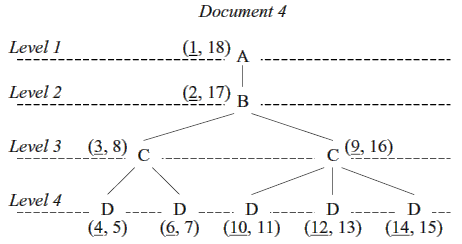
\includegraphics[width=2.7in]{img/numb.png}
\end{center}
\caption{Sample numbering of XML tree}
\label{fig:numb}
\end{figure}

Figure \ref{fig:numb} shows the numbering for the following document:

\begin{verbatim}
<A>
  <B>
    <C>
      <D>...</D>
      <D>...</D>
    </C>
    <C>
      <D>...</D>
      <D>...</D>
      <D>...</D>
    </C>
  </B>
</A>
\end{verbatim}

Start and end number appear as pairs, while the level appears on the left of the picture.
The start and end number actually represent the order of the opening and closing tag for
that element in the document, respectively. In order for the numbering to be consistent,
we assume that all \ldots\ that appear in the document represent text only (i.e., no more
tags). The start numbers are underlined because they also represents the identification
values for the elements. As a last remark, the number of the represented XML document\\
is assumed to be 4 (as shown in the picture).

\begin{figure}[ht]
\begin{center}
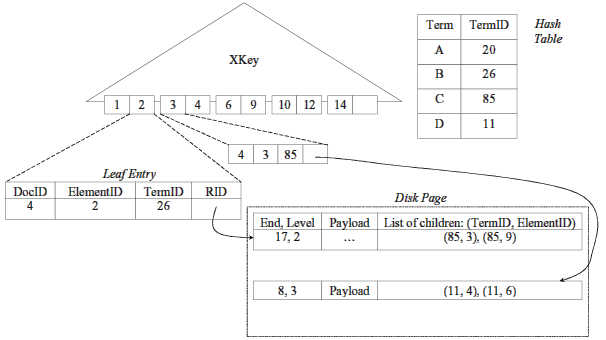
\includegraphics[width=3.5in]{img/dm.png}
\end{center}
\caption{Sample tree structure}
\label{fig:dm}
\end{figure}

In terms of data model, each XML document is stored using a B+-tree structure. The
structure that corresponds to the document from above appears in figure \ref{fig:dm}.
XKey is the name for the (document id, element id) pair which is used as the key in
the B+-tree (the element id is actually the start number you have seen in the numbering
scheme). Each leaf in the tree consists of an XKey and another two values: a \textbf{term
id} (which represents a hash value of the element name) and a \textbf{record id}
(which is a pointer to a location where all the information about the element can be
found). As you can see in the figure, each of the nine elements in the document (one
A, one B, two C's and 5 D's) has a corresponding leaf in the tree.

\begin{figure}[ht]
\begin{center}
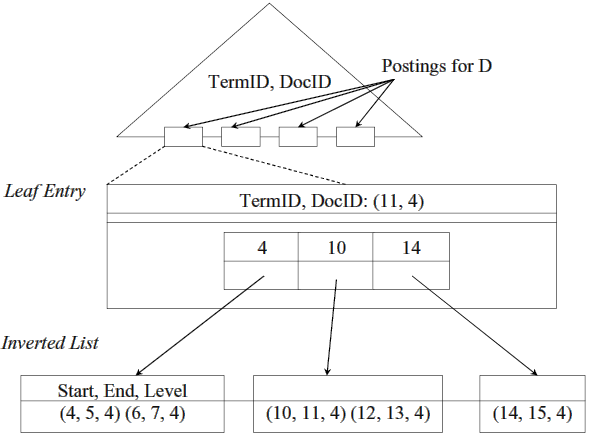
\includegraphics[width=3.7in]{img/im.png}
\end{center}
\caption{The index structure}
\label{fig:im}
\end{figure}

Now that the setting has been briefly covered, we can explain the index that is proposed
for such a structure. While the name and value indexes which we described in the previous
sections merely stored an inverted list for each element or value  (or just for some of them),
the posting list index will do more or less the same thing, with some distinctions:

\begin{itemize}
\item it will index based on the term id associated with an element name instead of the
element name itself
\item a posting list which consists of (start number, end number, level) triples, which
identify nodes in the tree indirectly (i.e., not by pointing at them), will be used instead
of an inverted list \item all the elements in the index will be stored in a B+-tree instead
of a linear list, so that scalable retrieval of nodes can be ensured
\end{itemize}

The index, as shown in figure \ref{fig:im}, is organized on two levels. The first one is a B+-tree
which uses pairs consisting of term id's and document id's as keys. Each leaf contains a
posting list, which is actually a (logical) inverted list enumerating occurrences of terms in
documents. Each such occurrence, called a posting, is represented by a (start number, end
number, level) triple in the posting list.

The second level index is used to provide indexed access to the postings in each posting list.
The entries in the posting list are stored in pages (or blocks, to make the connection to the
theory which we've studied in Database Architectures) and the index has an entry listing
the start number of the first posting in each page. It is thus a sparse index, built as a B+-tree,
for the postings based on their start numbers.

To further clarify figure \ref{fig:im}, I would like to mention that the four arrows labeled
as postings for D mean that each document (our example from above, Document 4, being
just one of the four shown here) has a posting list for D (and others for A, B, \ldots, not shown
in the image), consisting of all the postings of D in that particular document. What I am
trying to point out is that just one of the four posting lists (the one for which the
2\textsuperscript{nd} level index is also expanded) shown in the figure represents all
five occurrences of D from the sample document introduced earlier.

Now we can see how this index can be put to work by analyzing how an XQuery like

\begin{verbatim}
  doc("Document_4.xml")//D
\end{verbatim}

is processed. Since we are only searching for occurrences of D in Document 4, we will
use as key in the first level index the pair formed by associating the term id that corresponds
to D (i.e., 11, see the hash table from figure \ref{fig:dm}) with the document id that
corresponds to Document 4 (i.e., 4). This key is used to retrieve the entire posting list
for D in Document 4 and the list can then be used to get all occurrences of D from the
tree representing the XML document. If we want to retrieve the D elements from all
documents in a collection, by having an XQuery like

\begin{verbatim}
  collection("mydocs")//D
\end{verbatim}

we can use just the term id corresponding to D (again, 11) as the key in the top level index
to retrieve the posting lists for D in all the documents, not just in Document 4, and then
use them to find the actual nodes.

In order to see why the second level index is also useful, consider the document in figure
\ref{fig:zz} (represented directly as a tree). Suppose we need to provide an answer to the
following query:

\begin{figure}[ht]
\begin{center}
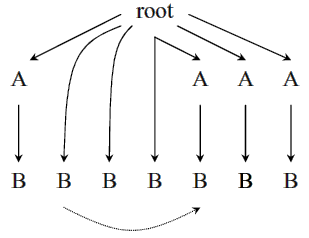
\includegraphics[width=2in]{img/zigzag.png}
\end{center}
\caption{Zig zag join on document}
\label{fig:zz}
\end{figure}

\begin{verbatim}
  doc("sample.xml")/A//B
\end{verbatim}

The request is to provide all those elements of type B which appear as part of an A element.
Effectively, if we have the posting list index available, this can be implemented as a join in
which we join all the elements in the posting list of A with all the elements in the posting list
of B and choose those elements from the result for which the (start number, end number)
interval of B is included in the (start number, end number interval) of the A it is joined with.
Let me emphasize here that the postings in the A posting list and in the B posting list are both
sorted in increasing order of the start number (because this is the way the index is created
and maintained).

To efficiently determine the right result, we can perform a sort of zig zag join algorithm in
which as soon, say, the current posting of A (i.e., the one currently examined in the join
process)  shows that the posting's end number is smaller than B's current posting's start
number, we can safely skip to the next posting in A's posting list, as we can be sure (due to
the increasing order of the start numbers in B's posting list) that no other posting in B's
posting list will join with this posting of A. This is the point where the second level index can
prove useful because it can allow us to skip entire pages of postings without checking all
the postings in these pages, but rather by simply noticing that the sparse index entries show,
for example, that all postings in a certain page of A's posting list have their end number
smaller than the B's current posting's start number. Since the index stores start numbers,
not end numbers, the way to notice what I was suggesting before is by looking at the index
of the page following the one that is to be skipped and seeing that the start number of the
first posting in that page is actually still smaller than B's current posting's start number.
This implies that no posting in the page to be skipped can have a higher end number.

In a similar manner (which will not be detailed here, as it should already be clear), the
current pointer in the B posting list can be moved as soon as it is detected that its end
number is smaller than A's current posting's start number, again by consulting the 2\textsuperscript{2n}
level index of B's posting list. This is shown in figure \ref{fig:zz} by the arrow in the lower
part of the figure.

This concludes than the presentation of the posting list index.

\section{Structural Indexes}
\label{sec:si}

A somewhat more advanced technique of building indexes on XML documents is one
which takes the (tree) structure of the XML document into account. The idea of all
structural indexes is to create a minimalized image of the structure which can be
used for faster access into the actual tree representing the XML document.

There has been a lot of research conducted on this topic, and in no way was it possible
for me to cover it all in such short time. Therefore, I have decided to adopt the following
strategy: I will characterize this entire class of indexes in a generic manner and then
very briefly enumerate some of the early attempts to propose such indexes and relate
them to this generic framework. Once this is done, I will then go into greater depth about
a solution which I have found to be particularly interesting.

\subsubsection*{Early Attempts}

Even though the representation of  a XML document is a tree, as some of the works
which I mention here were not necessarily based on XML or its data model, but also on
other types of semi structured data, the notion of graph will be rather encountered instead
of that of tree. This, however, is not really an issue since we know that every tree is
also a graph.

Kaushik et al. provide in \cite{kau04} a generic overview of what a \textit{structure index}
means, which I am going to explain here. Supposing we have a directed graph representing
an XML document (which is actually a tree, but, as I mentioned before, I am going to ignore
this slight inconsistency issue from here on), a structure index for this graph is yet another directed
graph which will actually be a summary of the original. By this I mean that it will preserve
all paths which exist in the original graph, but will only have one instance of each path,
as opposed to an unlimited number of instances which can appear in the original one. This
will naturally significantly decrease the number of nodes and edges of the index graph.

Each node in the index will have a certain extent associated with it. What this extent actually
is will differ from one structure index to the other but, generally speaking, it will be a
collection of nodes in the original XML data graph which is, by some particular mean
(e.g., by name), associated with the node in the index. What we are trying to do with
such an index is partition the elements in the original graph in such a way that an index
node can stand for an entire partition. Also, there has to be some logic behind creating
these partitions which makes the index useful for various types of XQuery's.

More formally speaking, citing \cite{kau04}, ``any partition of the element nodes
defines a structure index where we

\begin{enumerate}
\item associate an index node with every equivalence class,
\item define the \textit{extent} of each node $n$, $ext(n)$, to be the equivalence class
that formed it, and
\item add an edge from index node $A$ to index node $B$ if there is an edge from some
data node in $ext(A)$ to some data node in $ext(B)$.''
\end{enumerate}

Simply put, we consider that some nodes from the data graph are equivalent to one
another by defining some equivalence relationship, we partition the data graph according
to this relationship and associate an index node with each partition (or equivalence class)
we obtained as a result of this process. Then we ``draw'' edges between the index nodes
(which, remember, represent equivalence classes) if there are edges between members
of the equivalence classes themselves. An example of such an equivalence relationship is
to say that two data nodes are equivalent if they have the same label (i.e., they represent
elements with similar tag names). As a final remark, it should be pointed out that such
a structure index does not index the text nodes in a document, but only the element nodes.

The example which is used in the above quoted paper to illustrate structure indexes is reproduced
in what follows. Let us assume we want to index the document in figure \ref{fig:xmldt}. The result
of indexing this document using the label equivalence relationship is shown in figure
\ref{fig:xmlidx}. The numbers in red from the latter figure indicate the id's of the nodes they
are associated to in the index.

\begin{figure}[ht]
\begin{center}
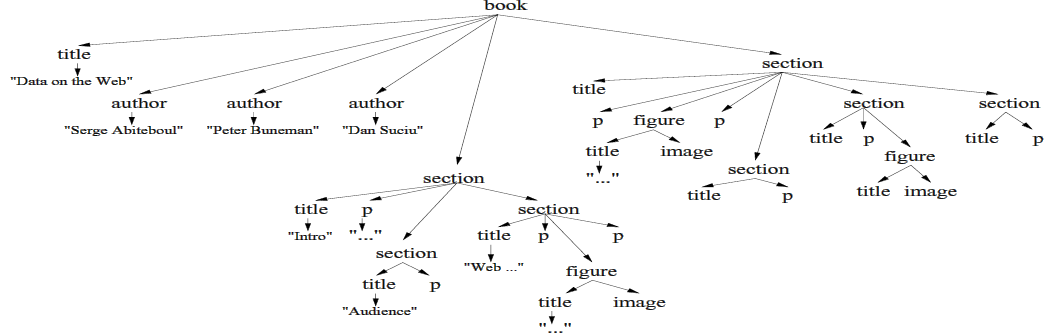
\includegraphics[width=\linewidth]{img/xmldt.png}
\end{center}
\caption{Sample XML data tree}
\label{fig:xmldt}
\end{figure}

\begin{figure}[ht]
\begin{center}
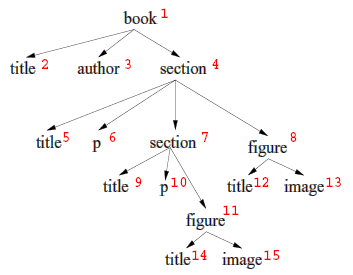
\includegraphics[width=2in]{img/xmlidx.png}
\end{center}
\caption{Structure index for the tree in figure \ref{fig:xmldt}}
\label{fig:xmlidx}
\end{figure}

The way such an index can be used is quite straightforward. If we need to execute a XQuery
like

\begin{verbatim}
  doc("sample.xml")/book/section/figure
\end{verbatim}

we can simply go into the index graph to the node indicated by this path in the tree and retrieve
the extent associated with this node. The extent will be exactly the result we are looking for. If,
on the other hand, we need to deal with an XQuery like

\begin{verbatim}
  doc("sample.xml")//section
\end{verbatim}

it is still useful (but perhaps not as useful as another structure could be) to have an index graph
associated with the XML data graph, because finding all nodes labeled ``section'' in the index graph
is much faster than the similar process in the data graph. This is due to the fact that the number of nodes
in the index graph is smaller (possibly orders of magnitude smaller, if the XML document has a
lot of structure repetition) than the one in the data graph. Once we have found all the nodes
labeled ``section'' in the index graph, we simply create a union of their extents in order to get
the result we need.

This is the general frame into which most early efforts fit. Surely, there will be distinctions
and extensions from one case to the other, but the general idea is still there. Here are, then, some
pointers to such work:

\begin{enumerate}

\item \textbf{Dataguides} are described in \cite{gol00} as ``concise and accurate structural
summaries of semi structured databases.'' They are also based on label equivalence and there is
just one path in the index graph for each similar path in the actual document. The formal definition
provided by the authors reads: ``A DataGuide for an OEM (Object Exchange Model) source object $s$
is an OEM object $d$ such that every label path of $s$ has exactly one data path instance in $d$, and
every label path of $d$ is a label path of $s$.'' Here, the XML data graph is referred to as the source
object ($s$) and the index graph is referred to as the destination object ($d$).

\item Three other structural indexes, the \textbf{1-Index}, the \textbf{2-Index} and the \textbf{T-index}
are proposed in \cite{mil97}. Actually, all three are based on the same idea, the distinction being that the
first one is appropriate for paths (in the tree) of length 1, the second one for paths of length 2 and the
third one for paths of any length. This idea of the template indexes (as they are actually called) is to
associate a T-index with a class of paths specified by a class template. Nodes in the data graph that are
the same with respect to a class of paths are grouped into equivalence classes and a T-index is then
associated to these classes.

\item The third paper on the list, \cite{kau02}, tries to extend on the previous idea of template indexes
by proposing something called a \textbf{forward and backward index} which should be able to handle
branching path expressions in addition to simple path expressions. The equivalence classes used here
are a bit more complex, but the idea is that 1-Index or dataguides are used on a modified version of the
original graph. The modification involves adding some more edges to the graph in order to provide some
inverse links between nodes (thus justifying the ``backward'' part of the index name).

\end{enumerate}

The papers listed above are just a small sample of a much larger ``research space''.

\subsubsection*{XPath Accelerator Index}

The author of \cite{gru02} proposes an index which, in contrast with the ones presented in the previous
subsection (as well as many others), is capable to support all XPath axes (XPath is a subset of the XQuery
language which is used by XQuery to express path selections wherever they are needed in an XQuery).
This feature, the author advertises, ``lets the index stand out among related work on XML indexing
structures which had a focus on regular path expressions (which correspond to the XPath axes \textit{children}
and \textit{descendant-self}) plus name tests.''

To understand axes in XPath, it is necessary to first have a look at how a XPath expression looks like.
In a simplified view, an XPath expression is an enumeration of node names preceded by some specification
of a tree on which the expression is to be evaluated. How these node names are related to one another
is defined by the axes which separate each pair of consecutive nodes in the enumeration. An XPath
expression is evaluated from left to right, in a step by step manner. Each step takes a set of nodes as
input and produces a set of nodes as output. Step $i$'s output set will become step $(i+1)$'s input set.
Every step will loop through its list of input nodes and, for each of them, produce a set of output nodes.
The resulting sets of output nodes of the step will be unioned together and sorted in document order\footnote[1]
{Document order is a central concept in XPath. Intuitively, it refers to the ordering of the
nodes in the data tree in such a way that the textual ordering of two elements in the original XML
document is preserved in the data tree. A formal definition of document order can be found in \cite{w3cdm}.}
to create the final output set. As each node in an input set is processed by a step, this node is called
the current \textit{context node} on which it is acted. Here is where the notion of \textit{axis} comes
into play. An axis determines how the context node is used to generate a new set of nodes, which is then
filtered according to the name of the element from the path expression. Some examples of axes are
\textit{child}, \textit{descendant}, \textit{ancestor-or-self}, \textit{following} or \textit{preceding-sibling}.
/ and // represent shorthand names for the \textit{child} and the \textit{descendant-or-self} axes,
respectively. These two axes are the ones that have been mainly addressed by the other index proposals.

The \textit{XPath accelerator} index structure is, as mentioned before, introduced by \cite{gru02} in
order to address the fact that XQuery's will need appropriate indexing for paths that also involve
other axes than / and //. The main observation which guided the author to the design of this index is
that a step's axis establishes a \textit{document region} in the document. Furthermore, if the established
document regions are analyzed, an interesting conclusion can be drawn, namely that four (of the total of
13 axes) together with the current context node cover the entire document without overlapping. These four
axes are the \textit{descendant}, \textit{ancestor}, \textit{following} and \textit{preceding} axes.
This is illustrated by the article using the following example. Consider the XML document from below:

\begin{verbatim}
<a>
  <b>
    <c>
      <d> </d><e> </e>
    </c>
  </b>
  <f>
    <g> </g>
    <h>
      <i> </i><j> </j>
    </h>
  </f>
</a>
\end{verbatim}

Figure \ref{fig:regions} then shows the regions for context node $f$ (taking into account that the
\textit{following} axis contains no nodes for context node $f$).

\begin{figure}[ht]
\begin{center}
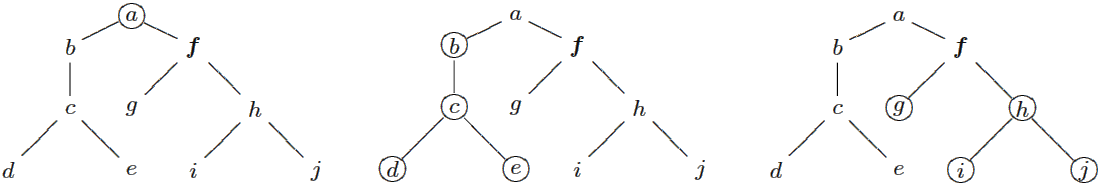
\includegraphics[width=\linewidth]{img/regions.png}
\end{center}
\caption{Circled nodes are elements of the regions defined by the \textit{ancestor}, \textit{descendant} and
\textit{preceding} axes, respectively, for context node $f$}
\label{fig:regions}
\end{figure}

The regions defined by any of the other axes except the four major ones mentioned above can
be obtained by performing various operations on the four regions defined by the major axes. In
addition to the remaining axes, also other features of the XPath language (such as predicates
on elements, for example) can be specified in terms of the four regions. This indicates that if
the four main regions can be indexed, then the rest of the problem will have a more or less
straightforward solution.

The remaining problem, then, is to provide an indexing method for these four regions. Another
useful observation here, which the author of \cite{gru02} himself takes from yet other authors,
is that if one defines two values for each node $v$, namely $pre(v)$ and $post(v)$, which represent
the index associated with the node if the data tree is traversed in pre- and post-order, respectively,
then these two values can be used to characterize the descendants $v'$ of $v$ as follows:\\

\begin{math}
v'\textmd{ is a descendant of }v
\Leftrightarrow
pre(v) < pre(v')\wedge post(v') < post(v)
\end{math}\\
\\
\indent{}This should be easily understood if one thinks of an XML sequence like
\tt $<$v$><$v'$>$\ldots$<$/v'$><$/v$>$\normalfont, where $<$v$>$ has to be seen before
$<$v'$>$ and $<$/v$>$ has to be seen after $<$/v'$>$ in order for $v'$ to be a descendant of
$v$. If, however, the nodes are placed into a plane which uses $pre$ as its $x$-axis and $post$
as its $y$-axis, then it can easily be seen that the two values will perfectly separate the four
regions we are interested in. This is also illustrated for the example which was introduced previously
in figure \ref{fig:prepost} (reproduced from \cite{gru02}).

\begin{figure}[ht]
\begin{center}
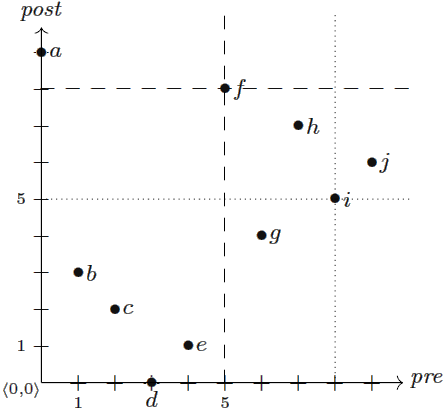
\includegraphics[width=3in]{img/prepost.png}
\end{center}
\caption{Node distribution in the $pre/post$ plane}
\label{fig:prepost}
\end{figure}

If you look at context node $f$, you will notice that the lower left region consists of the nodes in
the region defined by the \textit{preceding} axis, the lower right region consists of the nodes in the
region defined by the \textit{descendant} axis, the upper left region consists of the nodes in the
region defined by the \textit{ancestor} axis and the upper right region (had it not been empty)
would have consisted of the nodes in the region defined by the \textit{following} axis. The figure
explicitly shows the same division for the $i$ context node as well, while for the rest of the nodes
it can also be noticed.

Without going into details explaining why, I will just say that an additional number of three values
is necessary for each node so that the regions defined by the remaining axes, as well as by additional
constructs allowed by XPath, can be described in terms of the four main regions. These values, for
a node $v$, are

\begin{itemize}
\item $par(v)$ - the value of $pre$ for the parent of $v$
\item $att(v)$ - true, if node $v$ represents an attribute node, false otherwise
\item $tag(v)$ - the element tag or attribute name for node $v$
\end{itemize}

As a consequence, then, each node will have a descriptor associated with it, which is just a 5-tuple
containing all the values described above:\\

\begin{math}
desc(v) = \langle{}pre(v), post(v), par(v), att(v), tag(v)\rangle
\end{math}\\
\\
\indent{}Based on these five values, a query window can be described (and is described in \cite{gru02})
for each particular axis. Such query window will include a number of the node descriptors and, by
mapping to the node space, the nodes themselves. As a result, this model can be used to select
the groups of nodes which represent the answer to a certain step in the path. Naturally, by combining
these groups according to the evaluation method described earlier, an entire XPath expression can
be evaluated based on this index.

As node descriptors are elements in a 5-dimensional space, the author of \cite{gru02} suggests two
possible implementations for this index: one based on an R-tree and one based on 2 B-trees, one for
the $pre$ values and one for the $post$ values (the B-tree implementation is suggested to be used,
due to decreased performance, only if R-trees are not available).

Such an index is general enough to support any kind of XPath query. I believe that an example of
usage is not necessary, as it should have already become clear from the description how the index is
to be used. In a nutshell, for each evaluation step, the index can be used to identify the groups of
nodes that need to be considered in the next step, without any need of looking at the data tree.

\section{Conclusion}

This report has merely scratched the surface of the research that is being done in the field of
indexes for XML data. Even like that, I hope it has brought a certain amount of light over the
subject and that it can also prove to be useful as a starting point in investigating this area of
research. The kinds of indexes that are described in this paper can naturally be used in implementation
of XML databases, but I am sure that further analysis of papers or articles can reveal perhaps
even more interesting proposals.

\begin{thebibliography}{99}

\bibitem{cha04} Chamberlin, D., Draper, D., et al.: XQuery from the Experts - A Guide to the W3C XML Query Language.
Addison-Wesley, 2004.

\bibitem{gru02} Grust, T.: Accelerating XPath Location Steps.\\
\textit{http://www.inf.uni-konstanz.de/~grust/files/xpath-accel.pdf}

\bibitem{gol00} Goldman, R.; Widom, J.: DataGuides: Enabling Query Formulation and Optimization in Semistructured Databases.\\
\textit{http://www-db.stanford.edu/lore/pubs/dataguide.pdf}

\bibitem{hal03} Halverson, A., Burger, J., et al.: Mixed Mode XML Query Processing.\\
\textit{http://www.vldb.org/conf/2003/papers/S08P02.pdf}

\bibitem{kau02} Kaushik, R., Bohannon, P., et al.: Covering Indexes for Branching Path Queries.\\
\textit{http://www.cs.wisc.edu/~raghav/paper-309.pdf}

\bibitem{kau04} Kaushik, R., Krishnamurthy, R., et al.: On the Integration of Structure Indexes and Inverted Lists.\\
\textit{http://www.cs.wisc.edu/~sekar/application/struct-invlist.pdf}

\bibitem{mil97} Milo, T., Suciu, D.: Index Structures for Path Expressions.\\
\textit{http://www.math.tau.ac.il/~milo/ftp/icdt99-1.ps}

\bibitem{w3cdm} W3C: XQuery 1.0 and XPath 2.0 Data Model.\\
\textit{http://www.w3.org/TR/xpath-datamodel/}

\bibitem{w3cxq} W3C: XQuery 1.0: An XML Query Language.\\
\textit{http://www.w3.org/TR/xquery/}

\end{thebibliography}

\end{document}